%% TCDimerTreeTopology
%% FigS6TCDimerTreeTopology.tex
%% Unused packages and definitions removed; TikZ/PGFPlots source formatted.

\documentclass[tikz,margin=2mm]{standalone}
\usepackage{amssymb}
\usetikzlibrary{arrows}

\def\b{\mathsf{b}}
\def\c{\mathsf{c}}
\def\d{\mathsf{d}}

\begin{document}

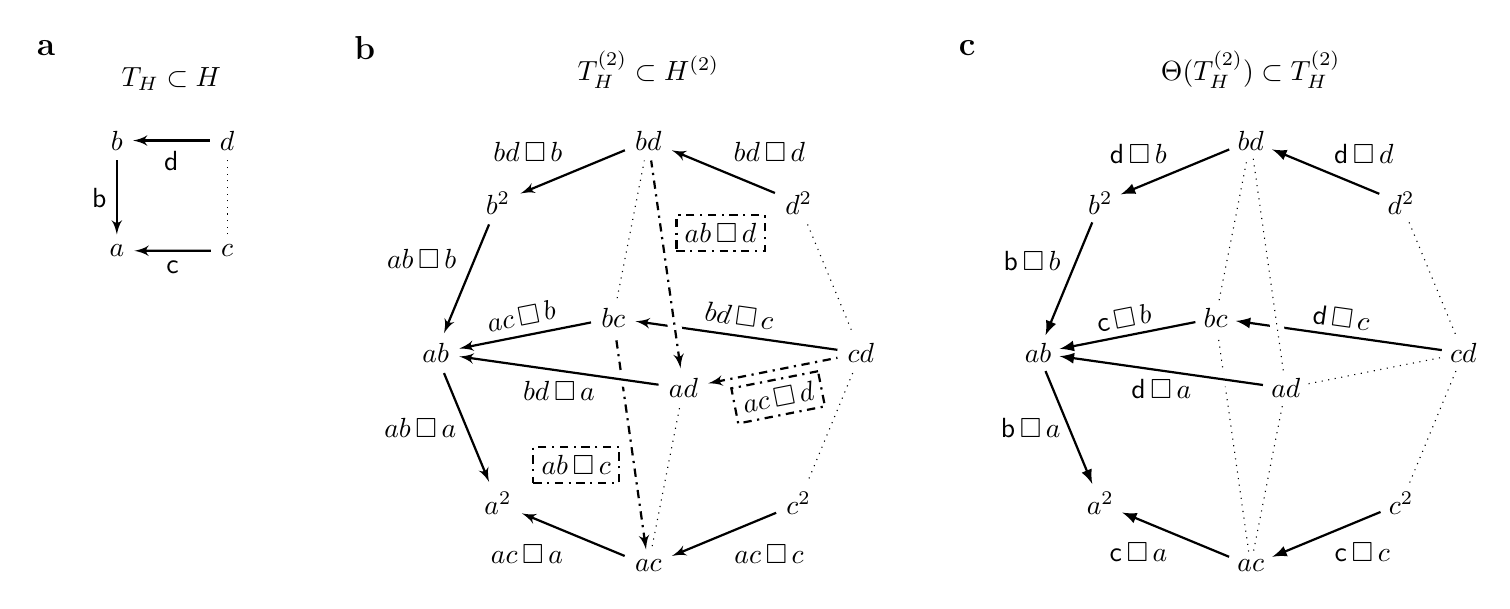
\begin{tikzpicture}[scale=0.9,style=thick,shorten >=0pt,shorten <=0pt,>=latex']

    \begin{scope}[node distance=1.4cm,xshift=-7cm,yshift=3cm]
        \node (B) {$b$};
        \node[below of=B] (A) {$a$};
        \draw[->,thick] (B) to node[left,align=center] {$\b$} (A);
        \node[right of=A] (C) {$c$};
        \draw[<-,thick] (A) to node[below] {$\c$} (C);
        \node[right of=B] (D) {$d$};
        \draw[->,thick] (D) to node[below] {$\d$} (B);
        \draw[dotted,thin] (C) to (D);
        \path (B) to node[above,yshift=0.5cm] {$T_H \subset H $} (D);
    \end{scope}

    \begin{scope}[xshift=0.5cm,yshift=0cm,scale=1,shorten >=0pt,shorten <=0pt]
        \coordinate (title) at (90:4);
        \draw (title) node {$T_H^{(2)} \subset H^{(2)}$};
        \draw (0:3) node[] (cd) {$cd$};
        \draw (45:3) node[] (d2) {$d^2$};
        \draw (90:3) node[] (bd) {$bd$};
        \draw (135:3) node[] (b2) {$b^2$};
        \draw (180:3) node[] (ab) {$ab$};
        \draw (225:3) node[] (a2) {$a^2$};
        \draw (270:3) node[] (ac) {$ac$};
        \draw (315:3) node[] (c2) {$c^2$};
        \draw (315:0.7) node[] (ad) {$ad$};
        \draw (135:0.7) node[] (bc) {$bc$};
        \draw[<-,thick] (a2) -- node[left] {$ab \, \Box \, a $} (ab);
        \draw[<-,thick] (ab) -- node[above left] {$ ab \, \Box \, b$} (b2);
        \draw[<-,thick] (b2) --  node[pos=0.75] (b2bd) {} node[above left] {$bd \, \Box \, b$} (bd);
        \draw[<-,thick] (bd) -- node[above right] {$bd \, \Box \, d$} (d2);
        \draw[thin,dotted] (d2) -- (cd);
        \draw[thin,dotted] (cd) -- (c2);
        \draw[<-,thick] (ac) -- node[below right] {$ac \, \Box \, c$} (c2);
        \draw[->,thick] (ac) -- node[below left] {$ac \, \Box \, a $} (a2);
        \draw[thin,dotted] (bc) -- (bd);
        \draw[thin,dotted] (ad) -- (ac);
        \draw[<-,thick] (ab) --  node[above,sloped] {$ac \, \Box \, b$} (bc);
        \draw[<-,thick] (bc) -- node[above,sloped] {$bd \, \Box \, c $} (cd);
        \draw[<-,thick,dashdotted] (ad) -- node[below,sloped,pos=0.5,draw,thick,dashdotted,inner sep=3pt,yshift=-3pt]  {$  ac \, \Box \, d $}  (cd);
        \draw[white,line width=5pt] (ad) -- node[pos=0.75] (adbd) {} (bd);
        \draw[<-,thick,dashdotted] (ad) -- node[pos=0.65,right,draw,thick,dashdotted,inner sep=3pt,xshift=5pt] (adbd) { $ ab \, \Box \, d$} (bd);
        \draw[<-, thick,dashdotted] (ac) -- node[left,pos=0.4,draw,thick,dashdotted,inner sep=3pt,xshift=-5pt] (bcac) {$ ab \, \Box \, c $} (bc);
        \draw[white,line width=5pt] (ab) -- node[below] {$bd \, \Box \, a $} (ad);
        \draw[<-,thick] (ab) -- node[below] {$bd \, \Box \, a $} (ad);
    \end{scope}

    \begin{scope}[xshift=9cm,yshift=0cm,scale=1,shorten >=0pt,shorten <=0pt,outer sep=1pt,inner sep=2pt,>=latex]
        \coordinate (title) at (90:4);
        \draw (title) node {$\Theta(T_H^{(2)}) \subset T_H^{(2)}$};
        \draw (0:3) node[] (cd) {$cd$};
        \draw (45:3) node[] (d2) {$d^2$};
        \draw (90:3) node[] (bd) {$bd$};
        \draw (135:3) node[] (b2) {$b^2$};
        \draw (180:3) node[] (ab) {$ab$};
        \draw (225:3) node[] (a2) {$a^2$};
        \draw (270:3) node[] (ac) {$ac$};
        \draw (315:3) node[] (c2) {$c^2$};
        \draw (315:0.7) node[] (ad) {$ad$};
        \draw (135:0.7) node[] (bc) {$bc$};
        \draw[<-,thick] (a2) -- node[left] {$\b \, \Box \, a $} (ab);
        \draw[<-,thick] (ab) -- node[above left] {$ \b \, \Box \, b$} (b2);
        \draw[<-,thick] (b2) --  node[pos=0.75] (b2bd) {} node[above left] {$\d \, \Box \, b$} (bd);
        \draw[<-,thick] (bd) -- node[above right] {$\d \, \Box \, d$} (d2);
        \draw[thin,dotted] (d2) -- (cd);
        \draw[thin,dotted] (cd) -- (c2);
        \draw[<-,thick] (ac) -- node[below right] {$\c \, \Box \, c$} (c2);
        \draw[->,thick] (ac) -- node[below left] {$\c \, \Box \, a $} (a2);
        \draw[thin,dotted] (bc) -- (bd);
        \draw[thin,dotted] (ad) -- (ac);
        \draw[<-,thick] (ab) --  node[above,sloped] {$\c \, \Box \, b$} (bc);
        \draw[<-,thick] (bc) -- node[above,sloped] {$\d \, \Box \, c $} (cd);
        \draw[thin,dotted] (ad) --  (cd);
        \draw[white,line width=5pt] (ad) -- node[pos=0.75] (adbd) {} (bd);
        \draw[thin,dotted] (ad) --  (bd);
        \draw[thin,dotted] (ac) --  (bc);
        \draw[white,line width=5pt] (ab) -- node[below] {$\d \, \Box \, a $} (ad);
        \draw[<-,thick] (ab) -- node[below] {$\d \, \Box \, a $} (ad);

    \end{scope}

    \def\height{4.3}
    \def\left{-8}
    \draw (\left,\height) node[font=\large] {{\bf a}};
    \draw (\left+4.5,\height) node[font=\large] {{\bf b}};
    \draw (\left+13,\height) node[font=\large] {{\bf c}};

\end{tikzpicture}

\end{document}

